\documentclass[11pt,a4paper]{article}

\usepackage[utf8]{inputenc}
\usepackage[T1]{fontenc}
\usepackage[spanish,es-nodecimaldot]{babel}
\usepackage{geometry}
\usepackage{amsmath}
\usepackage{amssymb}
\usepackage{booktabs}
\usepackage{array}
\usepackage{graphicx}
\usepackage{float}
\usepackage{hyperref}
\usepackage{tabularx}
\usepackage{enumitem}
\usepackage{xcolor}
\usepackage{caption}
\usepackage{natbib}
\usepackage{multirow}
\usepackage{url}

\geometry{margin=2.5cm}
\emergencystretch=1.5em
\hypersetup{
    colorlinks=true,
    linkcolor=blue!50!black,
    citecolor=blue!50!black,
    urlcolor=blue!50!black,
    pdftitle={Evolucion del control TD3 para protesis mioelectrica hasta el baseline valido de 8000 episodios},
    pdfauthor={Proyecto EMG Prosthesis TD3}
}

\newcolumntype{L}[1]{>{\raggedright\arraybackslash}p{#1}}
\newcolumntype{C}[1]{>{\centering\arraybackslash}p{#1}}
\newcolumntype{Y}{>{\raggedright\arraybackslash}X}

\title{\textbf{Evoluci\'on del Control TD3 para una Pr\'otesis Mioel\'ectrica}\\
\large Desde la reward heredada inicial hasta el baseline v\'alido refinado de 8000 episodios}
\author{Proyecto \texttt{EMG\_Prosthesis\_TD3}}
\date{22 de marzo de 2026}

\begin{document}

\maketitle

\begin{abstract}
Este informe reordena la historia experimental completa del proyecto de control mioel\'ectrico con TD3, desde su formulaci\'on base hasta el baseline v\'alido actual. El objetivo no es solo reportar el \'ultimo resultado, sino explicar c\'omo se lleg\'o a \'el y qu\'e partes del proceso siguen siendo t\'ecnicamente valiosas. La narrativa parte del art\'iculo base del proyecto, que plante\'o una observaci\'on de 44 dimensiones, un espacio de acci\'on continuo de cuatro motores y una reward multicomponente orientada a seguimiento proporcional \citep{fuertes2026continuous}. A partir de la auditor\'ia del repositorio se identificaron problemas en la reward heredada, en la coherencia temporal del entorno y, posteriormente, un bug cr\'itico del simulador que inmovilizaba la pr\'otesis. Ese hallazgo obliga a reinterpretar varias corridas intermedias como etapas de depuraci\'on y no como benchmark principal. Tras corregir el simulador y reentrenar el sistema con una formulaci\'on coherente basada en tracking MSE, regularizaci\'on de acci\'on y acci\'on efectiva cuantizada, se obtuvo primero un baseline v\'alido de 2000 episodios y, despu\'es, un baseline refinado a 8000 episodios. El mejor checkpoint auditado de esta corrida larga fue \texttt{Agent7250}, cuyo test de 50 simulaciones alcanz\'o \texttt{trackingMSE = 0.043045}, \texttt{trackingMAE = 0.160336}, \texttt{actionL2 = 0.596444}, \texttt{saturationFraction = 0.392086} y \(\Delta a\) L2 medio de \(0.321385\). El documento concluye que el proyecto ya dispone de un baseline s\'olido y defendible en simulaci\'on, y que la siguiente fase debe concentrarse en conservar ese tracking mientras se sigue reduciendo saturaci\'on y esfuerzo de control.
\end{abstract}

\section{Objetivo y alcance}

Este documento tiene cuatro prop\'ositos:
\begin{enumerate}[leftmargin=1.2cm]
    \item reconstruir la evoluci\'on t\'ecnica del proyecto desde el dise\~no inicial hasta el baseline actual;
    \item separar con claridad qu\'e resultados deben interpretarse como benchmark v\'alido y cu\'ales deben interpretarse como etapas de depuraci\'on;
    \item describir con formulaci\'on matem\'atica y trazabilidad de c\'odigo la configuraci\'on que hoy s\'i funciona;
    \item fijar el baseline operativo actual del proyecto en simulaci\'on.
\end{enumerate}

Todas las corridas descritas en este informe se realizaron en simulaci\'on, con dataset pregrabado y sin hardware activo durante entrenamiento ni test:
\begin{itemize}[leftmargin=1.2cm]
    \item \texttt{usePrerecorded = true},
    \item \texttt{simMotors = true},
    \item \texttt{connect\_glove = false}.
\end{itemize}

\section{Punto de partida: el baseline conceptual del proyecto}

El punto de partida conceptual del proyecto es el manuscrito \emph{Continuous Operation of a Myoelectric Hand Prosthesis using the TD3 Reinforcement Learning Algorithm} \citep{fuertes2026continuous}. Ese trabajo es importante porque fij\'o tres ideas fundacionales que siguen vigentes:
\begin{enumerate}[leftmargin=1.2cm]
    \item un problema de control continuo sobre cuatro motores con TD3;
    \item una observaci\'on compuesta por features EMG y realimentaci\'on de encoders;
    \item la necesidad de una reward cuidadosamente moldeada para evitar estrategias no proporcionales y \emph{reward hacking}.
\end{enumerate}

En el art\'iculo base, el estado se defini\'o con 44 dimensiones:
\begin{equation}
s_t^{\text{base}} =
\begin{bmatrix}
\phi_t \\
\mathrm{enc}_t
\end{bmatrix}
\in \mathbb{R}^{44},
\end{equation}
donde \(\phi_t \in \mathbb{R}^{40}\) contiene cinco features por cada uno de los ocho canales EMG, y \(\mathrm{enc}_t \in \mathbb{R}^{4}\) representa los encoders normalizados de los cuatro motores \citep{fuertes2026continuous}. El espacio de acci\'on tambi\'en se fij\'o desde el inicio como continuo:
\begin{equation}
a_t \in [-1,1]^4,
\end{equation}
y despu\'es se escal\'o a PWM mediante multiplicaci\'on por una velocidad m\'axima.

Ese baseline conceptual sigue siendo importante porque justific\'o el uso de TD3 para control continuo en una pr\'otesis mioel\'ectrica, en l\'inea con la literatura sobre control actor-critic determinista y tareas continuas de manipulaci\'on \citep{fujimoto2018td3,mathworks_td3_agent,chen2023review}. Sin embargo, el repositorio evolucion\'o m\'as all\'a de esa formulaci\'on inicial, y gran parte del trabajo reciente se centr\'o en limpiar la reward, hacer trazable el entorno y corregir problemas estructurales que el manuscrito no capturaba todav\'ia.

\section{Evoluci\'on t\'ecnica del repositorio hasta el baseline actual}

\subsection{Reward heredada y primeros problemas detectados}

La reward heredada del repositorio proven\'ia de una l\'ogica pensada para premiar direcci\'on correcta, castigar movimiento inverso e incentivar que el agente no se quedara quieto. Su estructura efectiva pod\'ia resumirse como:
\begin{equation}
r_t^{\text{legacy}}
=
\frac{1}{4}\sum_{i=1}^{4}
\left[
\rho(a_{t,i}, c_{t,i})
2 \cdot \mathbf{1}(\exists j: a_{t,j}\neq 0)
-k \, |p_{t,i} - y_{t,i}|
-\alpha \, |a_{t,i} - a_{t-1,i}|
\right],
\end{equation}
donde \(c_{t,i}\) representaba la direcci\'on ``correcta'' inferida por comparaci\'on entre posiciones consecutivas, \(p_{t,i}\) la posici\'on actual del motor y \(y_{t,i}\) la referencia.

La auditor\'ia del c\'odigo encontr\'o cuatro debilidades t\'ecnicas graves en esta formulaci\'on:
\begin{itemize}[leftmargin=1.2cm]
    \item la reward comparaba acciones como si fueran discretas, aunque TD3 generaba acciones continuas;
    \item exist\'ia memoria oculta entre episodios mediante variables persistentes;
    \item la reward se calculaba con incoherencia temporal dentro de \texttt{step};
    \item la escala final de la reward no quedaba alineada de forma clara con el objetivo f\'isico de tracking.
\end{itemize}

Estas observaciones son consistentes con la literatura de \emph{reward shaping}: una reward puede maximizarse sin inducir necesariamente el comportamiento deseado si sus t\'erminos est\'an mal escalados o no reflejan el objetivo real \citep{deng2025reward}. En el proyecto, eso se manifestaba en estrategias agresivas, poco proporcionales y muy sensibles a detalles de implementaci\'on.

\subsection{Transici\'on a tracking MSE y reward interpretable}

La primera gran mejora estructural consisti\'o en reemplazar la reward heredada por una reward expl\'icita basada en error de tracking MSE normalizado y penalizaci\'on de magnitud de acci\'on. La formulaci\'on intermedia qued\'o:
\begin{equation}
r_t^{\text{MSE}}
=
-
\frac{1}{4}\sum_{i=1}^{4}
\left(
e_{t,i}^{2}
\lambda_a \tilde{a}_{t,i}^{2}
\right),
\end{equation}
con:
\begin{equation}
e_{t,i} = \hat{y}_{t,i} - y_{t,i},
\end{equation}
donde \(\hat{y}_{t,i}\) es la flexi\'on estimada de la pr\'otesis en la escala del glove y \(\tilde{a}_{t,i}\) es la acci\'on efectiva normalizada.

La decisi\'on de usar MSE fue coherente con dos criterios:
\begin{itemize}[leftmargin=1.2cm]
    \item penaliza con m\'as fuerza errores grandes, lo que es deseable en tracking continuo;
    \item proporciona una se\~nal densa y estable para TD3, a diferencia de rewards m\'as discretas o ambiguas \citep{fujimoto2018td3,mathworks_td3_options}.
\end{itemize}

En esta etapa tambi\'en se corrigieron la evaluaci\'on doble de reward dentro de \texttt{step} y el \emph{logging} por episodio, incorporando variables como \texttt{trackingMse}, \texttt{trackingMae}, \texttt{actionL2}, PWM aplicado y, m\'as adelante, variaci\'on de acci\'on.

\subsection{Remapeo a acci\'on efectiva y cuantizaci\'on expl\'icita}

La siguiente mejora importante consisti\'o en alinear la acci\'on aprendida por TD3 con la acci\'on realmente aplicable por el simulador. El actor segu\'ia produciendo:
\begin{equation}
a_t \in [-1,1]^4,
\end{equation}
pero esa acci\'on se remapeaba a un conjunto discreto de PWM efectivos:
\begin{equation}
\mathcal{U}_{\mathrm{PWM}} = \{0, 64, 96, 128, 160, 192, 224, 255\}.
\end{equation}

Esta intervenci\'on fue necesaria porque el simulador cuantizaba la acci\'on de hecho, y si el entorno no hac\'ia expl\'icita esa cuantizaci\'on, el agente pod\'ia aprender acciones peque\~nas que matem\'aticamente parec\'ian correctas pero f\'isicamente eran casi nulas. Esa alineaci\'on entre acci\'on continua y actuaci\'on efectiva es relevante en tareas prot\'esicas y de manipulaci\'on continua \citep{done2025prostheticrl,deng2025reward}.

\subsection{Ramas diagn\'osticas: progreso, 52D, 132D y TD3 recurrente}

Entre la transici\'on inicial a MSE y el baseline final se exploraron varias ramas:
\begin{itemize}[leftmargin=1.2cm]
    \item reward con t\'ermino de progreso y suavidad;
    \item observaci\'on Markoviana ampliada a 52D con delta de encoder y acci\'on previa;
    \item apilado temporal de EMG hasta 132D;
    \item TD3 recurrente con LSTM.
\end{itemize}

Estas ramas siguen siendo valiosas como ingenier\'ia exploratoria porque ayudaron a entender el papel de la memoria, de la acci\'on previa y de la suavidad. Tambi\'en est\'an bien motivadas por la literatura: la regularizaci\'on de suavidad puede ayudar en control rob\'otico \citep{lee2024smoothness}; y el contexto temporal es relevante en control mioel\'ectrico \citep{chen2023review}. Sin embargo, estas comparativas no deben tomarse como benchmark principal, porque ocurrieron antes de corregir el bug cr\'itico del simulador. Por tanto, hoy se interpretan como una l\'inea de aprendizaje del equipo y no como evidencia definitiva sobre la mejor arquitectura.

\section{Hallazgo cr\'itico: el simulador estaba inm\'ovil}

El punto de inflexi\'on real del proyecto fue el hallazgo de un bug estructural en el simulador. La auditor\'ia mostr\'o dos problemas:
\begin{enumerate}[leftmargin=1.2cm]
    \item la din\'amica basada en \texttt{fit\_C2.mat} se apoyaba en series \texttt{ws} vac\'ias, por lo que la pr\'otesis quedaba inm\'ovil aunque el agente enviara acci\'on;
    \item dentro de \texttt{step}, el tiempo del episodio se actualizaba despu\'es de leer la pr\'otesis, introduciendo un desfase temporal de un paso.
\end{enumerate}

Estas dos fallas explican por qu\'e varias corridas previas mostraban pol\'iticas visualmente extra\~nas o poco conclusivas: el agente estaba optimizando rewards y se\~nales internas del entorno, pero no estaba controlando una din\'amica f\'isica efectiva.

Se aplicaron dos correcciones m\'inimas y de bajo riesgo:
\begin{itemize}[leftmargin=1.2cm]
    \item en el simulador de la pr\'otesis, cuando \texttt{ws} est\'a vac\'io se usa \texttt{pattern\_curve.mat} como respaldo din\'amico;
    \item en \texttt{@Env/step.m}, el tiempo del episodio se adelanta antes de leer la pr\'otesis.
\end{itemize}

Este hallazgo obliga a una decisi\'on metodol\'ogica importante: las corridas pre-fix no deben usarse como benchmark num\'erico principal. S\'i deben conservarse como parte de la historia del proyecto, porque gracias a ellas se limpiaron reward, entorno, logging y pipeline. Pero el baseline operativo actual solo puede construirse a partir de corridas post-fix.

\section{Formulaci\'on v\'alida actual del problema}

\subsection{Observaci\'on actual}

La formulaci\'on v\'alida actual usa una observaci\'on Markoviana de 52 dimensiones:
\begin{equation}
s_t =
\begin{bmatrix}
\phi_t \\
\mathrm{enc}_t \\
\Delta \mathrm{enc}_t \\
\tilde{a}_{t-1}
\end{bmatrix}
\in \mathbb{R}^{52},
\end{equation}
donde:
\begin{itemize}[leftmargin=1.2cm]
    \item \(\phi_t \in \mathbb{R}^{40}\) son las features EMG del instante actual;
    \item \(\mathrm{enc}_t \in \mathbb{R}^{4}\) son los encoders normalizados;
    \item \(\Delta \mathrm{enc}_t \in \mathbb{R}^{4}\) es el cambio de encoder entre pasos;
    \item \(\tilde{a}_{t-1} \in [-1,1]^4\) es la acci\'on efectiva previa.
\end{itemize}

Esta formulaci\'on extiende el estado de 44D del art\'iculo base \citep{fuertes2026continuous} sin incorporar la referencia del glove como observaci\'on, lo cual preserva una interpretaci\'on correcta del problema: el agente debe inferir el control a partir de EMG y estado mec\'anico, no a partir del error ya calculado.

\subsection{Reward actual}

La reward actual es:
\begin{equation}
r_t =
-
\frac{1}{4}\sum_{i=1}^{4}
\left(
e_{t,i}^{2}
+
\lambda_a \tilde{a}_{t,i}^{2}
+
\lambda_{\Delta a}\left(\tilde{a}_{t,i} - \tilde{a}_{t-1,i}\right)^2
\right),
\label{eq:currentreward}
\end{equation}
con:
\begin{equation}
e_{t,i} = \hat{y}_{t,i} - y_{t,i},
\end{equation}
\(\lambda_a = 0.01\) y \(\lambda_{\Delta a} = 0.05\).

Esta reward representa la versi\'on madura de la l\'inea iniciada con MSE:
\begin{itemize}[leftmargin=1.2cm]
    \item el t\'ermino dominante sigue siendo tracking MSE;
    \item la magnitud de acci\'on evita soluciones de energ\'ia arbitraria;
    \item la penalizaci\'on de \(\Delta a\) favorece suavidad de control.
\end{itemize}

El dise\~no es coherente con el uso de TD3 en control continuo \citep{fujimoto2018td3,mathworks_td3_agent}, con literatura de \emph{reward shaping} en manipulaci\'on \citep{deng2025reward} y con trabajos recientes de regularizaci\'on de suavidad \citep{lee2024smoothness}.

\subsection{TD3 e hiperpar\'ametros del baseline actual}

La configuraci\'on vigente del baseline se resume en la Tabla~\ref{tab:td3-valid-8000}. Esta configuraci\'on se mantuvo constante a lo largo de la corrida larga de 8000 episodios; no se mezclaron cambios adicionales de arquitectura ni de reward durante ese refinamiento.

\begin{table}[H]
\centering
\caption{Configuraci\'on TD3 del baseline v\'alido refinado}
\label{tab:td3-valid-8000}
\small
\renewcommand{\arraystretch}{1.15}
\begin{tabularx}{\textwidth}{L{4.6cm}C{2.4cm}Y}
\toprule
\textbf{Par\'ametro} & \textbf{Valor} & \textbf{Interpretaci\'on} \\
\midrule
Observation variant & markov52 & Estado actual con contexto motor m\'inimo expl\'icito \\
State length & 52 & 40 features EMG + 4 encoders + 4 deltas + 4 acciones previas \\
Reward type & \texttt{trackingMseAction\-RateReward} & Tracking MSE + penalizaci\'on de acci\'on y de cambio de acci\'on \\
Reward action weight & 0.01 & Penaliza energ\'ia excesiva \\
Reward delta-action weight & 0.05 & Penaliza cambios bruscos \\
Actor / critics & MLP & Arquitectura simple y estable tras la correcci\'on del entorno \\
Hidden units & 64 & Capacidad media, suficiente para el problema actual \\
Actor learning rate & \(10^{-4}\) & Conservador para la pol\'itica \\
Critic learning rate & \(10^{-3}\) & Mayor para estimaci\'on de valor \\
Discount factor \(\gamma\) & 0.95 & Horizonte efectivo coherente con episodios cortos \\
Target smooth factor \(\tau\) & 0.005 & Actualizaci\'on lenta de redes objetivo \\
Mini-batch size & 64 & Compromiso entre estabilidad y eficiencia \\
Replay buffer & \(10^5\) & Suficiente para la escala actual \\
Exploration std & 0.2 & Exploraci\'on moderada \\
Target policy std & 0.2 & \emph{Policy smoothing} en TD3 \\
Checkpoint frequency & 250 & Resoluci\'on suficiente para una corrida larga de 8000 episodios \\
\bottomrule
\end{tabularx}
\end{table}

\section{Baseline v\'alido inicial post-fix: la corrida de 2000 episodios}

Despu\'es de corregir el simulador, la primera evidencia v\'alida apareci\'o con la corrida de 2000 episodios. Esa corrida no es ya el baseline final, pero sigue siendo importante porque demostr\'o que el sistema, con el entorno corregido, s\'i pod\'ia aprender tracking real. Sus resultados de test de 50 simulaciones fueron:
\begin{itemize}[leftmargin=1.2cm]
    \item \texttt{trackingMSE = 0.052805},
    \item \texttt{trackingMAE = 0.179093},
    \item \texttt{actionL2 = 0.674957},
    \item \texttt{saturationFraction = 0.474999},
    \item \(\Delta a\) L2 medio \(= 0.633264\).
\end{itemize}

Ese resultado fue el primer benchmark defendible del proyecto. Su importancia hist\'orica no es menor: marca el punto en el que el proyecto deja de estudiar artefactos del entorno y empieza a estudiar un problema genuino de control.

\section{Refinamiento del baseline: corrida de 8000 episodios}

\subsection{Resumen de entrenamiento}

La corrida larga de refinamiento se ejecut\'o en la carpeta \texttt{26-03-22 10 5 40}. La Figura~\ref{fig:train8000} muestra la evoluci\'on de \texttt{EpisodeReward}, \texttt{AverageReward} y \texttt{EpisodeQ0}. A diferencia de la corrida inicial de 2000 episodios, la mejora continu\'o apareciendo en la parte tard\'ia del entrenamiento, lo que justific\'o el aumento de presupuesto.

\IfFileExists{figures/training_progress_8000eps_valid_baseline.png}{
\begin{figure}[H]
\centering
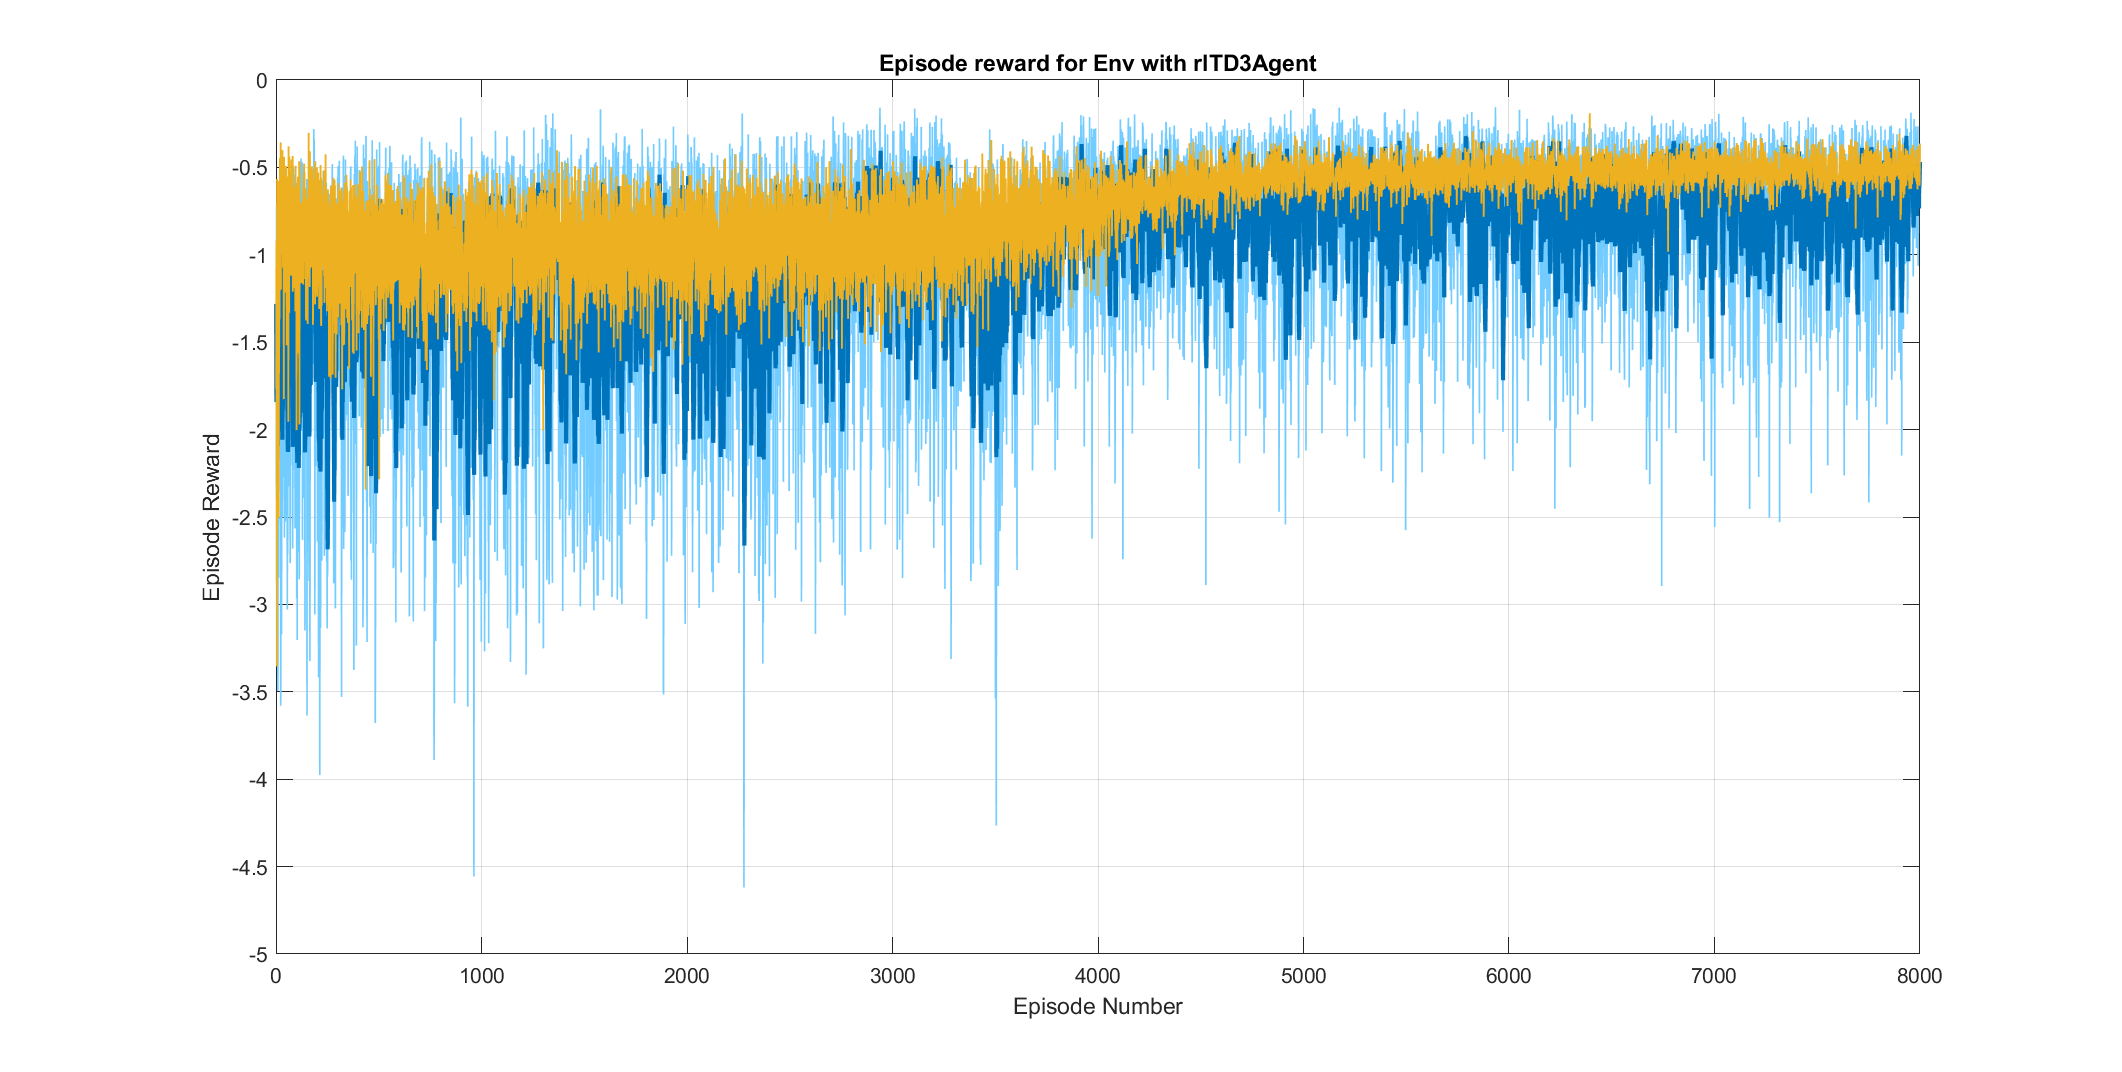
\includegraphics[width=\textwidth]{figures/training_progress_8000eps_valid_baseline.png}
\caption{Corrida larga v\'alida de 8000 episodios. La mejora del promedio m\'ovil contin\'ua hasta la zona del episodio 7934, lo que indica que el agente segu\'ia refinando el control.}
\label{fig:train8000}
\end{figure}
}{}

El resumen cuantitativo de la corrida completa se presenta en la Tabla~\ref{tab:train8000-summary}.

\begin{table}[H]
\centering
\caption{Resumen cuantitativo de la corrida larga v\'alida de 8000 episodios}
\label{tab:train8000-summary}
\small
\renewcommand{\arraystretch}{1.15}
\begin{tabularx}{\textwidth}{L{5.8cm}C{2.6cm}Y}
\toprule
\textbf{M\'etrica} & \textbf{Valor} & \textbf{Lectura} \\
\midrule
EpisodeReward medio & \(-0.9779\) & Mejor que el baseline v\'alido inicial de 2000 episodios \\
EpisodeReward final & \(-0.4860\) & El final de la corrida sigue siendo competitivo \\
Best EpisodeReward & \(-0.1554\) en ep. 5934 & Persisten episodios muy buenos tambi\'en en la parte media-tard\'ia \\
AverageReward final & \(-0.4687\) & El promedio final mejora de forma clara sobre el baseline de 2000 episodios \\
Best AverageReward & \(-0.3195\) en ep. 7934 & El mejor tramo aparece casi al final de la corrida \\
TrackingMSE medio & \(0.0612\) & Error de entrenamiento bajo y estable \\
TrackingMAE medio & \(0.1914\) & Error absoluto consistente con la mejora sostenida \\
ActionL2 medio & \(0.4672\) & Menor esfuerzo medio que en el baseline inicial v\'alido \\
Saturation fraction & \(0.1992\) & La saturaci\'on en entrenamiento cae de forma importante \\
\(\Delta a\) L2 medio & \(0.1811\) & La pol\'itica se suaviza durante el entrenamiento \\
\bottomrule
\end{tabularx}
\end{table}

La lectura t\'ecnica de esta tabla es importante: la corrida de 8000 no solo mejor\'o reward, sino tambi\'en suavidad y saturaci\'on media durante entrenamiento. Eso sugiere una mejora real de la pol\'itica y no simplemente una versi\'on m\'as agresiva del agente anterior.

\subsection{Auditor\'ia de checkpoints de la cola}

Aunque el mejor promedio apareci\'o cerca del episodio 7934, no se asumi\'o que \texttt{Agent8000} fuera el mejor checkpoint. Se audit\'o la cola de la corrida con una evaluaci\'on r\'apida de 20 simulaciones por checkpoint. Los resultados se muestran en la Tabla~\ref{tab:tail8000}.

\begin{table}[H]
\centering
\caption{Auditor\'ia r\'apida de checkpoints de la parte final de la corrida de 8000 episodios}
\label{tab:tail8000}
\small
\renewcommand{\arraystretch}{1.12}
\begin{tabularx}{\textwidth}{L{2.4cm}C{1.8cm}C{1.8cm}C{1.8cm}C{1.8cm}C{1.8cm}Y}
\toprule
\textbf{Checkpoint} & \textbf{MSE} & \textbf{MAE} & \textbf{ActionL2} & \textbf{Sat.} & \textbf{\(\Delta a\)} & \textbf{Lectura} \\
\midrule
Agent5750 & 0.046003 & 0.166895 & \textbf{0.502443} & \textbf{0.294033} & 0.333084 & Muy conservador, tracking competitivo \\
Agent6000 & 0.044541 & 0.164541 & 0.569580 & 0.358387 & 0.346737 & Mejora tracking, algo m\'as agresivo \\
Agent7250 & \textbf{0.043045} & \textbf{0.160336} & 0.596444 & 0.392086 & 0.321385 & Mejor tracking de la cola auditada \\
Agent7500 & 0.044390 & 0.163515 & 0.561740 & 0.333164 & 0.338822 & Similar a 6000, ligeramente inferior a 7250 \\
Agent7750 & 0.043835 & 0.162426 & 0.595294 & 0.365436 & 0.336460 & Muy competitivo, apenas por debajo de 7250 \\
Agent8000 & 0.044311 & 0.162612 & 0.530379 & 0.318648 & \textbf{0.298875} & Final muy estable, pero no el mejor en tracking \\
\bottomrule
\end{tabularx}
\end{table}

La decisi\'on de fijar \texttt{Agent7250} como mejor checkpoint es t\'ecnicamente razonable por dos motivos:
\begin{itemize}[leftmargin=1.2cm]
    \item obtuvo el menor \texttt{trackingMSE} de la cola auditada;
    \item no fue el m\'as agresivo de los candidatos cercanos, por lo que el mejor tracking no se consigui\'o simplemente empujando a m\'axima saturaci\'on.
\end{itemize}

\subsection{Test final de 50 simulaciones con \texttt{Agent7250}}

El test final se ejecut\'o con \texttt{Agent7250}. La Figura~\ref{fig:test7250} muestra el episodio 49, que es representativo del comportamiento observado.

\IfFileExists{figures/test_episode_49_valid_baseline_8000.png}{
\begin{figure}[H]
\centering
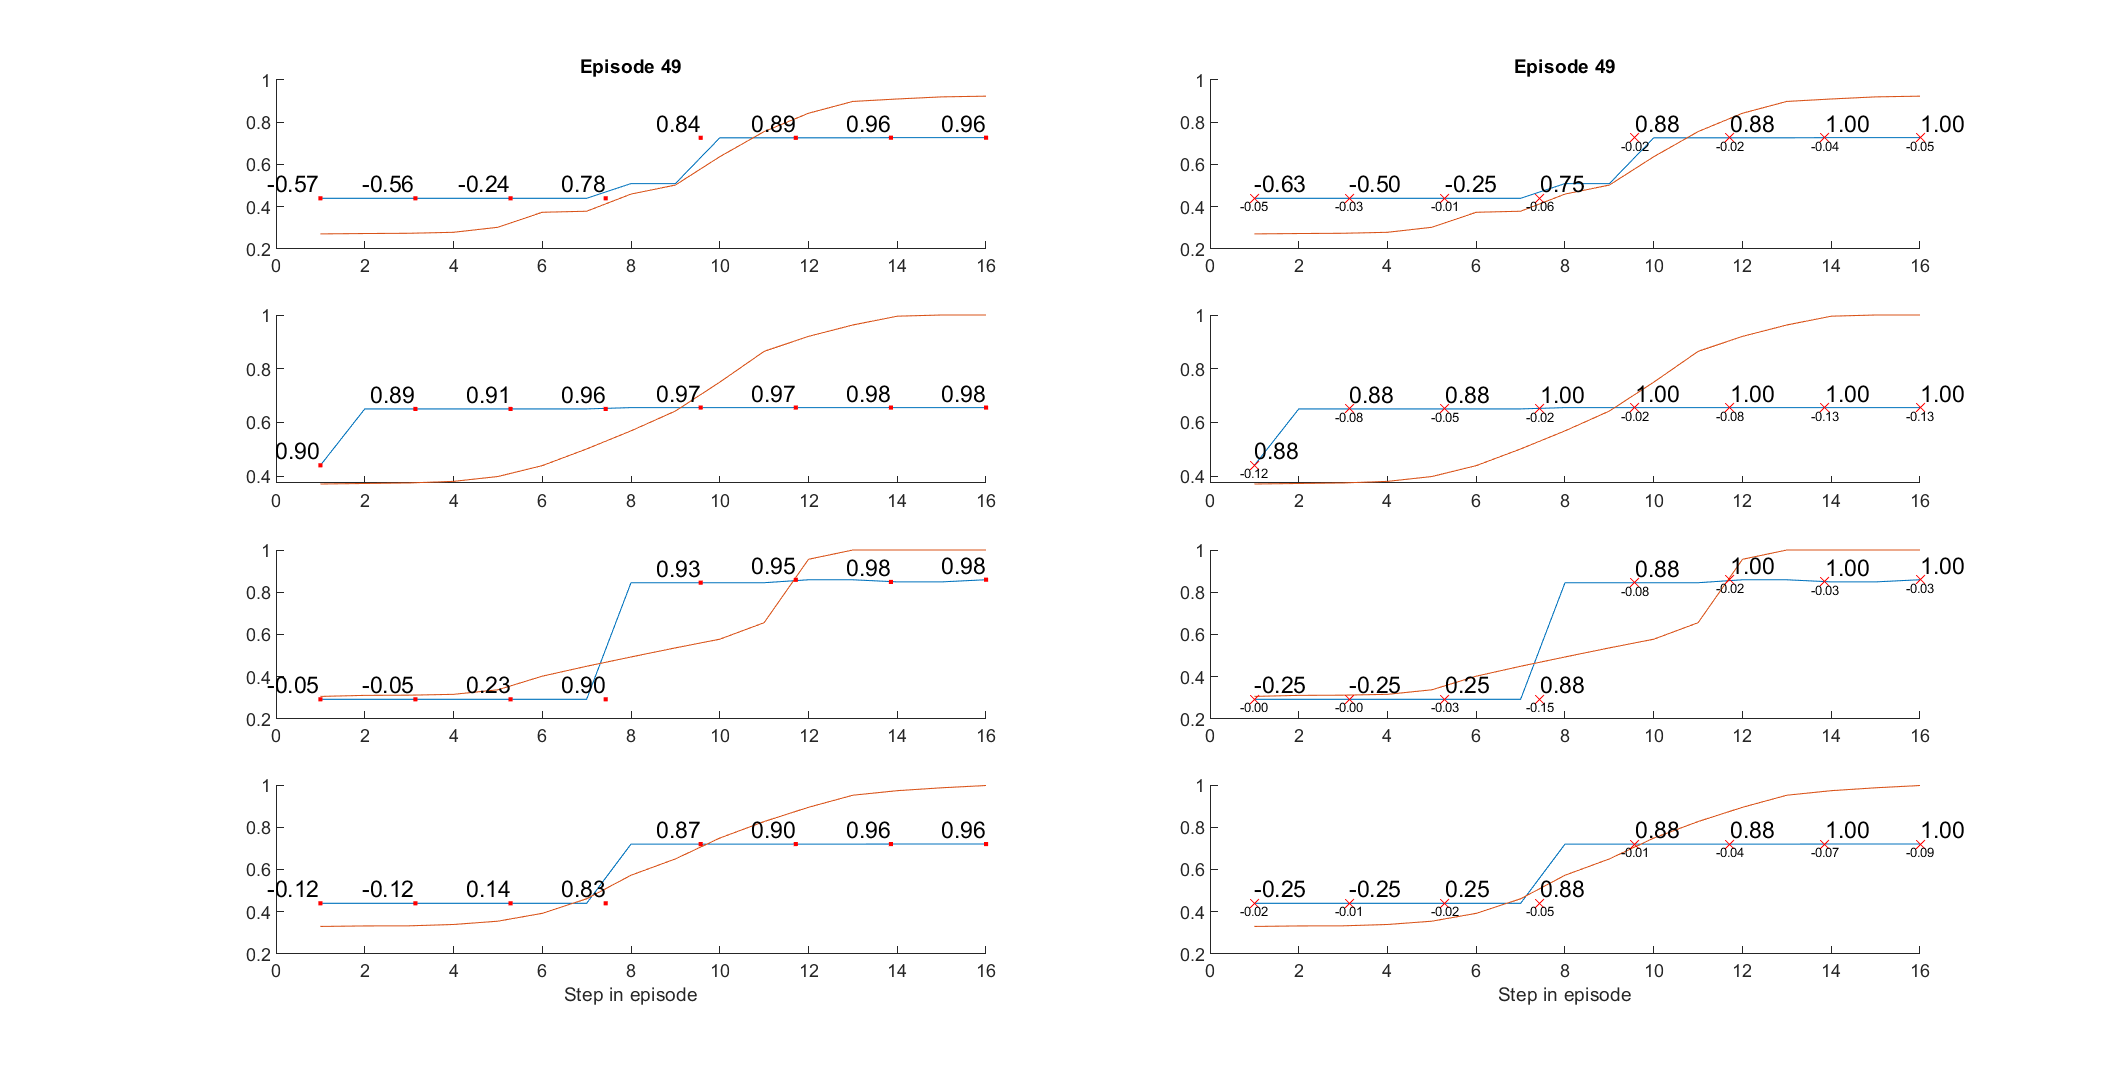
\includegraphics[width=\textwidth]{figures/test_episode_49_valid_baseline_8000.png}
\caption{Episodio 49 del test final con \texttt{Agent7250}. La trayectoria azul acompa\~na la referencia naranja con mayor fidelidad que el baseline v\'alido inicial, y lo hace con menor saturaci\'on global.}
\label{fig:test7250}
\end{figure}
}{}

Las m\'etricas agregadas del test se muestran en la Tabla~\ref{tab:test7250}.

\begin{table}[H]
\centering
\caption{Resumen del test final de 50 simulaciones con \texttt{Agent7250}}
\label{tab:test7250}
\small
\renewcommand{\arraystretch}{1.15}
\begin{tabularx}{\textwidth}{L{5.3cm}C{2.5cm}Y}
\toprule
\textbf{M\'etrica} & \textbf{Valor} & \textbf{Interpretaci\'on} \\
\midrule
TrackingMSE medio & \(0.043045\) & Nuevo mejor tracking v\'alido del proyecto en simulaci\'on \\
TrackingMAE medio & \(0.160336\) & Error absoluto medio claramente mejor que el baseline inicial v\'alido \\
ActionL2 medio & \(0.596444\) & Menor energ\'ia de control que el baseline de 2000 episodios \\
PWM absoluto medio & \(178.288566\) & El agente sigue siendo activo, pero menos extremo que el baseline inicial \\
Fracci\'on de saturaci\'on & \(0.392086\) & Saturaci\'on todav\'ia importante, pero menor que antes \\
\(\Delta a\) L2 medio & \(0.321385\) & La acci\'on es mucho m\'as suave que en el baseline inicial \\
\bottomrule
\end{tabularx}
\end{table}

\subsection{Comparaci\'on v\'alida: 2000 episodios vs 8000 episodios}

La comparaci\'on v\'alida m\'as importante del proyecto no es con las ramas pre-fix, sino entre el primer baseline post-fix de 2000 episodios y el baseline refinado de 8000 episodios. Esa comparaci\'on se resume en la Tabla~\ref{tab:valid-comparison}.

\begin{table}[H]
\centering
\caption{Comparaci\'on entre el baseline v\'alido inicial y el baseline refinado actual}
\label{tab:valid-comparison}
\small
\renewcommand{\arraystretch}{1.15}
\begin{tabularx}{\textwidth}{L{3.8cm}C{2.2cm}C{2.2cm}Y}
\toprule
\textbf{M\'etrica} & \textbf{Agent2000} & \textbf{Agent7250} & \textbf{Lectura} \\
\midrule
TrackingMSE & 0.052805 & \textbf{0.043045} & Mejora aproximada del 18.5\% \\
TrackingMAE & 0.179093 & \textbf{0.160336} & Mejora aproximada del 10.5\% \\
ActionL2 & 0.674957 & \textbf{0.596444} & Menor esfuerzo total \\
Saturation fraction & 0.474999 & \textbf{0.392086} & Menor saturaci\'on efectiva \\
\(\Delta a\) L2 & 0.633264 & \textbf{0.321385} & Pol\'itica mucho m\'as suave \\
PWM absoluto medio & 195.913207 & \textbf{178.288566} & Menor uso del extremo alto del actuador \\
\bottomrule
\end{tabularx}
\end{table}

Esta es la comparaci\'on que hoy s\'i debe usarse para defender el estado del proyecto. Muestra que aumentar el presupuesto a 8000 episodios, manteniendo la formulaci\'on actual, no solo mejor\'o tracking sino tambi\'en el compromiso tracking--agresividad. Esa es una conclusi\'on mucho m\'as fuerte que la que se ten\'ia en el baseline inicial.

\section{Qu\'e sigue siendo \'util de las etapas previas}

Aunque las ramas pre-fix no deban usarse como benchmark num\'erico principal, s\'i dejaron aprendizaje t\'ecnico acumulado que sigue vigente:
\begin{itemize}[leftmargin=1.2cm]
    \item la auditor\'ia de reward fue correcta: la reward heredada deb\'ia ser sustituida por una reward expl\'icita y densa;
    \item la incorporaci\'on de \textit{logging} detallado por episodio fue crucial para detectar mejoras reales;
    \item el remapeo de acci\'on efectiva fue una intervenci\'on necesaria y permanece en el baseline actual;
    \item las ramas de 52D, 132D y TD3 recurrente sirvieron para descartar hip\'otesis y entender mejor la relaci\'on entre observabilidad, memoria y suavidad.
\end{itemize}

En otras palabras, esas etapas no se pierden: pasan de ser ``comparativas finales'' a ser ``trabajo de ingenier\'ia que hizo posible el baseline actual''.

\section{Veredicto t\'ecnico actual}

El estado actual del proyecto puede resumirse en cinco afirmaciones:
\begin{enumerate}[leftmargin=1.2cm]
    \item el proyecto parte de una l\'inea base conceptualmente s\'olida basada en TD3, observaci\'on EMG y control continuo \citep{fuertes2026continuous};
    \item la reward heredada del repositorio deb\'ia ser reemplazada, y la transici\'on a MSE fue una decisi\'on correcta;
    \item las comparativas intermedias anteriores al fix del simulador deben interpretarse como evoluci\'on t\'ecnica, no como benchmark definitivo;
    \item tras corregir el simulador, el baseline de 52 dimensiones demostr\'o que el proyecto s\'i pod\'ia aprender tracking real;
    \item la corrida de 8000 episodios refin\'o ese baseline y fij\'o a \texttt{Agent7250} como mejor agente operativo actual.
\end{enumerate}

Por tanto, el proyecto ya no est\'a en una fase de ``exploraci\'on incierta'' sino en una fase de optimizaci\'on fina sobre una base v\'alida.

\section{L\'inea futura recomendada}

La siguiente etapa no deber\'ia volver a cambiar observaci\'on, reward y arquitectura a la vez. Ahora que existe un baseline v\'alido y refinado, la l\'inea de menor riesgo es:
\begin{enumerate}[leftmargin=1.2cm]
    \item conservar la observaci\'on Markoviana de 52 dimensiones;
    \item mantener TD3 y el remapeo de acci\'on efectiva;
    \item estudiar ajustes finos de \(\lambda_a\) y \(\lambda_{\Delta a}\) para reducir saturaci\'on sin perder el tracking logrado;
    \item auditar checkpoints de nuevas corridas largas para no asumir que el \'ultimo episodio es el mejor;
    \item dejar arquitecturas m\'as complejas o estrategias h\'ibridas para una etapa posterior y ya sobre un benchmark estable.
\end{enumerate}

Esta l\'inea es coherente con la literatura. TD3 sigue siendo adecuado para control continuo \citep{fujimoto2018td3,mathworks_td3_agent}; la suavidad de acci\'on es una propiedad deseable en rob\'otica \citep{lee2024smoothness}; y en pr\'otesis mioel\'ectricas la estabilidad y la interpretabilidad de la se\~nal de control son tan importantes como el error medio puro \citep{chen2023review,done2025prostheticrl}.

\section{Conclusi\'on}

La conclusi\'on correcta del proyecto ya no es que ``TD3 podr\'ia servir'' ni que ``el reward parece razonable''. La conclusi\'on correcta es mucho m\'as fuerte: el proyecto ha recorrido una secuencia completa de depuraci\'on, redise\~no de reward, alineaci\'on de acci\'on efectiva, detecci\'on y correcci\'on de un bug cr\'itico de simulaci\'on, y refinamiento experimental hasta llegar a un baseline v\'alido y cuantitativamente mejorado.

En esa historia, el baseline conceptual del art\'iculo inicial \citep{fuertes2026continuous} fue importante porque fij\'o la direcci\'on del problema. La auditor\'ia del repositorio fue importante porque mostr\'o que el reward original y el entorno ten\'ian incoherencias. Las ramas intermedias fueron importantes porque ense\~naron qu\'e hip\'otesis no bastaban por s\'i solas. Pero el punto verdaderamente decisivo fue la correcci\'on del simulador. A partir de ah\'i, el baseline de 2000 episodios demostr\'o que el sistema s\'i aprend\'ia. Y la corrida de 8000 episodios demostr\'o que ese aprendizaje pod\'ia refinarse hasta mejorar simult\'aneamente tracking, esfuerzo, saturaci\'on y suavidad.

Ese es el estado actual del proyecto: no un prototipo especulativo, sino un baseline serio en simulaci\'on sobre el cual ya tiene sentido seguir mejorando.

\bibliographystyle{plainnat}
\bibliography{references}

\end{document}
